\chapter{Experiments}

\section{Corpus Statistics}
\begin{table}[H]
	\centering
	\begin{tabular}{c|c|c|c|c}
		\hline
		\multirow{4}{*}{\textbf{Train}} & \textbf{}              & \textbf{German} & \textbf{English} & \textbf{French} \\ \cline{2-5} 
		& \textbf{Sentences}     & \textbf{100M}   & \textbf{100M}    & \textbf{100M}   \\ \cline{2-5} 
		& \textbf{Running Words} & \textbf{1880M}  & \textbf{2360M}   & \textbf{3017M}  \\ \cline{2-5} 
		& \textbf{Vocabulary}    & \textbf{1254k}  & \textbf{523k}    & \textbf{660k}   \\ \hline
	\end{tabular}
	
\end{table}

\begin{table}[H]
	\centering
	
	\begin{tabular}{c|c|c|c|c|c}
		\hline
		\multirow{7}{*}{\textbf{Test}} & \textbf{}                      & \multicolumn{2}{c|}{\textbf{\texttt{newstest2016}}}    & \multicolumn{2}{c}{\textbf{\texttt{newstest2014}}}    \\ \cline{3-6} 
		& \multicolumn{1}{l|}{\textbf{}} & \textbf{German}       & \textbf{English}      & \textbf{French}       & \textbf{English}      \\ \cline{2-6} 
		& \textbf{Sentences}             & \textbf{2999}         & \textbf{2999}         & \textbf{3003}         & \textbf{3003}         \\ \cline{2-6} 
		& \textbf{Running Words}         & \textbf{62506}        & \textbf{64619}        & \textbf{81165}        & \textbf{71290}        \\ \cline{2-6} 
		& \textbf{Vocabulary Size}       & \textbf{11978}        & \textbf{8645}         & \textbf{10899}        & \textbf{9200}         \\ \cline{2-6} 
		& \textbf{OOV Rates}             & \textbf{4116 (6.6\%)} & \textbf{1643 (2.5\%)} & \textbf{1731 (2.1\%)} & \textbf{1299 (1.8\%)} \\ \cline{2-6} 
		& \textbf{LM perplexity}         & \textbf{211.0}        & \textbf{109.6}        & \textbf{51.2}         & \textbf{84.6}         \\ \hline
		\multicolumn{4}{l}{\textbf{Search vocabulary in testing: 50k (src/tgt)}} \\
		
	\end{tabular}
\end{table}
\section{Word Translation}
\subsection{Baseline Experiments}
 \cite{conneau2017word} release high-quality dictionaries for 12 oriented language pairs; a train and test split of 5000 and 1500 unique source words for each language pair. We train the monolingual word embedding with fastText(\cite{bojanowski2016enriching}) and compare the performances of different training methods for word retrieval upon this dataset. As demonstrated in Table , CSLS performs better than other dictionary induction methods like simple nearest neighbour search (NN)  or inverted softmax (ISF). So in all tables related to word retrieval task, CSLS is the default method if without any specification.

\begin{table}[H]
	\centering
	\begin{tabular}{llccc}
		\hline
		\multicolumn{2}{l}{Methods}                           & NN    & ISF   & CSLS  \\ \hline
		Supervised                    & Procrustes             & 60.37 & 63.22 & 65.38 \\ \hline
		\multirow{2}{*}{Unsupervised} & Adversarial            & 47.03 & 49.57 & 53.50 \\ \cline{2-5} 
		& Adversarial+Procrustes & 61.75 & 62.68 & 64.92 \\ \hline
	\end{tabular}
\end{table}
\subsubsection{Vocabulary Size for Word Translation}


\subsection{Corpus-based Approach}
We run the novel corpus-based approach on a relative small corpus with 50k sentences using different learning rate schedulers; one is to start from initial learning rate, the other is to inherit the learning rate after the training of last batch sentences. The first learning rate scheduler always performs better than the second one. We demonstrate the results for German$\rightarrow$ English and English $\rightarrow$ German for the first scheduler. In order to lift the performance of the second scheduler, we augment training corpus by training two loops over the 50k corpus and extend the corpus size to 200k. The results get better but still worse than that with first learning rate scheduler. 
\subsubsection{Different Learning Rate Scheduler}
\begin{itemize}
	\item Start from Initial Learning Rate
	\begin{itemize}
		\item Word translation accuracies for German$\rightarrow$English,  with different initial learning rates and sentence batch sizes.
		\begin{table}[H]
			\centering
			\begin{tabular}{cccccc}
				\hline
				Accuracy (\%) & 100   & 500   & 1k    & 2k    & 5k    \\ \hline
				0.01          & 1.00  & 6.01  & 24.21 & 28.37 & 42.71 \\ \hline
				0.005         & 0.85  & 5.47  & 7.71  & 17.12 & 38.78 \\ \hline
				0.001         & 1.23  & 7.32  & 14.88 & 15.34 & 27.45 \\ \hline
				0.0005        & 1.54  & 45.26 & 49.88 & 54.43 & 54.97 \\ \hline
				0.0001        & 36.23 & 58.09 & 60.14 & 60.37 & 58.67 \\ \hline
			\end{tabular}
%		\caption{Word translation accuracy for German $\rightarrow$ English}
		\end{table}
		\item Word translation accuracy for English $\rightarrow$ German, with different initial learning rates and sentence batch sizes.
		\begin{table}[H]
			\centering
			\begin{tabular}{cccc}
				\hline
				Accuracy (\%) & 1k   & 2k   & 5k      \\ \hline
				0.01          & 10.02  & 16.50  & 23.36 \\ \hline
				0.005       & 47.65 & 22.28 & 24.21 \\ \hline
				0.001        & 24.44 & 24.98 & 26.75 \\ \hline
				0.0005          & 54.82  & 55.67  & 48.44 \\ \hline
				0.00001        & 59.21 & 58.98 & 56.90 \\ \hline
			\end{tabular}
%		 \caption{Word translation accuracy for English $\rightarrow$ German}
		\end{table}	

		
	\end{itemize}
	\item Inherit Last Learning Rate
	\begin{itemize}
		\item Word translation accuracy for German$\rightarrow$English with different initial learning rates and sentence batch sizes.\\
		\begin{table}[H]
			\centering
			\begin{tabular}{cccc}
				\hline
				Accuracy (\%) & 1k   & 2k   & 5k      \\ \hline
				0.01          & 7.79  & 4.70  & 6.01 \\ \hline
				0.005       & 3.39 & 12.03 & 8.94 \\ \hline
				0.001        & 5.40 & 11.49 & 18.89 \\ \hline
				0.0005          & 5.78  & 8.33  & 10.25 \\ \hline
				0.00001        & 51.50 & 37.63 & 15.27 \\ \hline
			\end{tabular}
			%		\caption{Word translation accuracy for German$\rightarrow$English }
		\end{table}	
		\item Word translation accuracy for German$\rightarrow$English with different training corpus, initial learning rate $0.0001$ and batch size $1k$\\
		\begin{table}[H]
			\centering
			\begin{tabular}{lc}
				\hline
				Train & Accuracy (\%) \\ \hline
				50k   & 51.50         \\ \hline
				50k $\times$ 2 & 55.51         \\ \hline
				200k  & 57.87         \\ \hline
			\end{tabular}
			%	\caption{Word translation accuracy for German$\rightarrow$English on different training corpus}
		\end{table}
	\end{itemize}

	

\end{itemize}

\begin{figure}[H]
	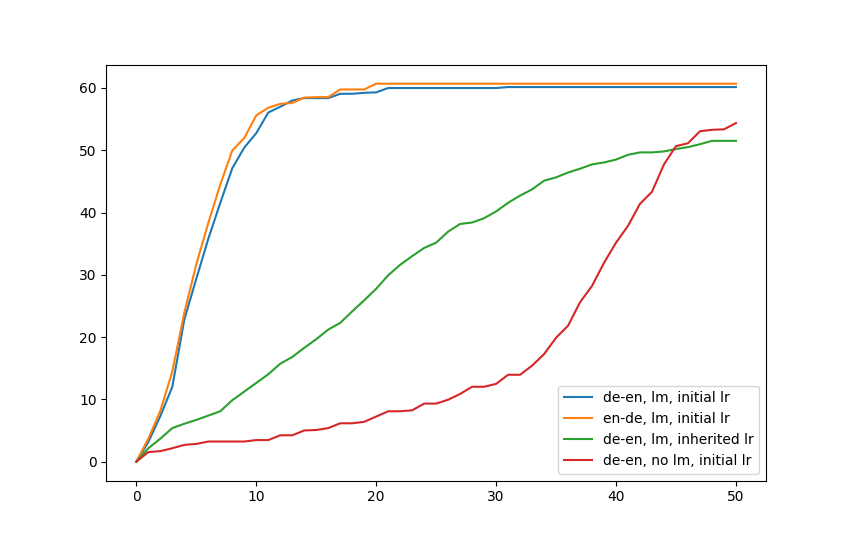
\includegraphics[width=14cm]{corpus}
	\centering
	\caption{A cross-lingual embedding space between German and English (\cite{ruder2017survey})}
\end{figure}


\section{Sentence Translation}


\subsection{Comprehensive Table}
\begin{table}[H]
	
%	\caption{Translation results on German$\leftrightarrow$English \texttt{newstest2016} and French$\leftrightarrow$English \texttt{newstest2014} }
	\centering
\scalebox{0.8}{
		\begin{tabular}{>{\bfseries}l>{\bfseries}c>{\bfseries}c>{\bfseries}c>{\bfseries}c}
			\toprule
			& De-En & En-De & Fr-En & En-Fr\\
			System   & \textsc{Bleu} [\%] & \textsc{Bleu} [\%] & \textsc{Bleu} [\%] & \textsc{Bleu} [\%]\\
			\midrule
			Word-by-Word   & 11.1 & 6.7 & 10.6 & 7.8\\
			\midrule
			+ LM (5-gram) + tgt w/ high LM score for OOV  & 12.9 & 8.9 & 12.7 & 10.0\\
			+ LM (5-gram) + copy from src for OOV		& 14.5 & 9.9 & 13.6 & 10.9\\
			\midrule
			\hspace{10pt}+ Denoising (RNN)  & 16.2 & 10.6 & 15.8 & 13.3 \\
			\hspace{10pt}+ Denoising (Transformer) & \leavevmode\color{blue}{17.2} & \leavevmode\color{blue}{11.0}& \leavevmode\color{blue}{16.5} & \leavevmode\color{blue}13.9 \\
			\midrule
			\cite{lample2017unsupervised} & 13.3 & 9.6 & 14.3 & 15.1\\
			\cite{artetxe2017unsupervised} & - & - & 15.6 & 15.1\\
			\bottomrule
		\end{tabular}
	}
\end{table}
As demonstrated above, our unsupervised MT surpass the start-of-the-art unsupervised NMT in almost all cases except English$\rightarrow$French translation. Each sub-model lift the performance respectively. Copy OOV word from source sentences works better than those predicted by language model, because OOV words are usually specific name entities and LM prefers common words rather than rare words. Denoising autoencoder based on Transformer structure outputs better translation than the traditional RNN structure. 


	\begin{table}[!h]
	\centering
	\caption {Word-by-word translation from German to English}
	\begin{tabular}{>{\bfseries}c>{\bfseries}c>{\bfseries}c}
		\hline
		&\textsc{Accuracy} [\%]& \textsc{Bleu} [\%] \\ \hline
		5M & 44.9  & 9.7  \\ \hline
		10M & 51.6 & 10.1 \\ \hline
		50M & 59.4 & 10.8 \\ \hline
		100M &\leavevmode\color{blue}61.2 & \leavevmode\color{blue}11.2 \\ \hline
	\end{tabular}
\end{table}


\subsection{BPE vs Word}
Byte pair encoding (BPE) is a simple data compression technique for word segmentation. It allows for the representation of an open vocabulary through a fixed-size vocabulary of variable-character sequences, making it very suitable word segmentation strategy for neural network models. It helps to reduce the vocabulary size and they eliminate the presence of unknown words in the output translation. We use BPE to represent the mapping between languages. 
	\begin{table}[h]
	\centering
	\scalebox{0.9}{
		\begin{tabular}{>{\bfseries}l>{\bfseries}c>{\bfseries}c}
			\toprule
			\multicolumn{2}{c}{\textbf{Vocabulary}} & \textsc{Bleu} [\%] \\
			\midrule
			& Merges \\
			\cmidrule{2-2}
			\multirow{3}{*}{BPE} & 
			20k & 10.4 \\
			& 50k & 12.5 \\
			& 100k & \leavevmode\color{blue}13.0 \\
			\midrule
			& Cross-lingual training \\
			\cmidrule{2-2}
			\multirow{4}{*}{Word} & 20k & 14.4\\
			& 50k & 14.4\\
			& 100k & \leavevmode\color{blue}14.5\\
			& 200k & 14.4\\
			\bottomrule
		\end{tabular}
	}\\

\end{table}


As the experiments results demonstrated above, the BPE performs worse than word in this unsupervised learning scenario. It might be difficult to learn the translation relationship between subword units. 

\subsection{Artificial Noise}

	\begin{table}[H]
	\centering
	\scalebox{1}{
		\begin{tabular}{>{\bfseries}c>{\bfseries}c>{\bfseries}c>{\bfseries}r>{\bfseries}c}
			\toprule
			$d_\text{per}$ & $p_\text{del}$ & $p_\text{ins}$ & $V_\text{ins}$ & \textsc{Bleu} [\%] \\
			\midrule
			2 & & & & 14.7\\
			3 & & & & \leavevmode\color{blue}{14.9}\\
			5 & & & & 14.9\\
			\midrule
			\multirow{2}{*}{3} & 0.1 & &  & \leavevmode\color{blue}{15.7} \\
			& 0.3 & & & 15.1 \\
			\midrule
			\multirow{4}{*}{3} & \multirow{4}{*}{0.1} & \multirow{4}{*}{0.1} & 10 & 16.8 \\
			& & & 50 & \leavevmode\color{blue}{17.2} \\
			& & & 500 & 16.8 \\
			& & & 5000 & 16.5\\
			\bottomrule
		\end{tabular}
	}
	\setcounter{table}{1}
	\label{tab:denoising}
\end{table}
Each artificial noise improves the translation performance, though the permutation noise only aims at local reordering instead of global reordering.




\subsection{Phrase Embedding}

\begin{table}[h]
	\centering
	\begin{tabular}{>{\bfseries}c>{\bfseries}c>{\bfseries}c>{\bfseries}c>{\bfseries}c  >{\bfseries}c}
		\hline
		\multicolumn{3}{c}{\multirow{2}{*}{\textbf{Vocabulary}}}                  & No LM & With LM & Denoising \\
		\multicolumn{3}{c}{}                                         &  \textsc{Bleu} [\%]  &  \textsc{Bleu} [\%] & \textsc{Bleu} [\%]   \\ \hline
		Word            & \multicolumn{2}{l}{}              & 11.2 & 14.5  &\leavevmode\color{blue}{ 17.2} \\
		\hline
		\multirow{3}{*}{\cite{mikolov2013distributed} } & \multirow{3}{*}{threshold} & 100  & 11.1 & 13.7  & 15.6 \\ \cline{3-6} 
		&                            & 500  & 11.0 & 13.7  & 16.2 \\ \cline{3-6} 
		&                            & 2000 & 10.7 & 14.0  &16.5 \\ \hline
		Top frequent              & \multicolumn{1}{l}{\textbf{count}}  & 50k  & \leavevmode\color{blue}12.0 & \leavevmode\color{blue}15.7  & 16.8 \\ \hline
	\end{tabular}
\end{table}

?????? not sure if I need to add this corresponding part in unsupervised cross-lingual embedding


%\subsection{Vocabulary Cutoff in Translation}
%\begin{table}[h]
%	\parbox{.5\linewidth}{
%		\centering
%		\caption{Word embedding vocabulary cut-off}
%		\begin{tabular}{>{\bfseries}c >{\bfseries}c >{\bfseries}c >{\bfseries}c } 
%			\hline
%			\textsc{Bleu} [\%]	& 20k & 50k & 100k \\
%			\hline
%			50k &	11.1  & \leavevmode\color{blue}11.3 & 11.2  \\ 
%			\hline
%			100k&	11.2  & 11.2 & 11.1 \\ 			
%			\hline
%			150k&	10.9 & 10.9 & - \\
%			\hline
%		\end{tabular}
%		
%	}
%	\hfill
%	\parbox{.5\linewidth}{
%		\centering
%		\caption{Phrase embedding vocabulary cut-off}
%		\begin{tabular}{>{\bfseries}c >{\bfseries}c >{\bfseries}c >{\bfseries}c } 
%			\hline
%			\textsc{Bleu} [\%]	& 50k & 100k & 150k \\
%			\hline
%			50k &	11.3  & - & -  \\ 
%			\hline
%			100k&	11.9  & 11.9 & - \\ 			
%			\hline
%			150k&	\leavevmode\color{blue}12.0 & 11.9 & 11.9 \\
%			\hline
%			200k & 12.0 & - & - \\
%			\hline
%		\end{tabular}
%		
%	}
%\end{table}
